\documentclass{article}
\usepackage[utf8]{inputenc}
\usepackage{xcolor}
\usepackage{url}
\usepackage[nottoc]{tocbibind}
\usepackage{graphicx}
\usepackage[bottom]{footmisc}
\usepackage{float}

\title{CSCE 479/879 Homework 1: [HW 1: Classifying Fashion MNIST + CIFAR-100]}
\author{Shubham Bery \\
Shiva Paudel \\
Puranjit Singh \\
Kantilata Thapa} 
%\date{February 2022}

\begin{document}

\maketitle

\begin{abstract} 
For this homework, our team developed deep learning models for the Fashion MNIST and CIFAR-100 datasets. The focus of this homework was to understand the intuition and working of deep neural networks and how tuning/tweaking of different hyperparameters affect models’ capability to generalize better on unseen data. Fashion MNIST dataset has grayscale images; we trained two different architectures with fully connected layers on this dataset.The maximum validation accuracy for this dataset was 0.89 with the 95\% confidence intervals for the generalization error of (0.1024, 0.1145) and for CIFAR 100 datasets we got validation accuracy of 39\% which was highest with 40\% dropout and L2 regularization between dense layers. The total number of images in the CIFAR-100 and Fashion-MNIST dataset are same. Since, Cifar 100 has a higher number of classes in which the whole dataset is splitted, which leads to a less number of images per each class. This makes it challenging to develop a highly efficient model. To overcome this, we explored different architectures and hyperparameters. To make the network adapt to the domain of CIFAR-100, we also explored the potential of residual blocks in the network which enhanced the training and improveed validation accuracies. 

\end{abstract}

\section{Introduction}
\label{sec:intro}

Deep Learning has a wide variability of applications among various branches of science. Machine learning algorithms make use of predetermined equations in learning features from data, whereas deep learning algorithms use neural networks, to learn useful and representative features directly from the data without relying on a predetermined equations. Image classification is one subset of deep learning that is being used in different situations across industries. Classifying an image can be something trivial for a human eye but it poses a huge challenge for a machine to interpret an image. This is where the technologies like deep learning come in.\par
In this homework, Fashion-MNIST and CIFAR-100 datasets were used to train deep neural networks. Among the two datasets, CIFAR 100 had more complex data with 100 classes so it required a deeper convolution neural network. We used only fully connected Dense layers to develop deep learning model for Fashion-MNIST data and on the other hand convolutional and pooling layers were used in development of deep neural networks on Cifar 100 dataset.  Two different model architectures were used for both the datasets with hyperparameter tuning. For the Fashion MNIST dataset, our model performed better in second architecture having 10 hidden layers, 20\% dropout, 0.0001 learning rate along with L2 regularization at each dense layer. The validation accuracy was found to be 89\% with a validation loss of 0.4 which was comparatively lower compared to first architecture. For CIFAR-100 dataset, we managed to get the highest validation accuracy of 39\% with 40\% dropout and L2 regularization between dense layers. It was observed that for the fashion MNIST dataset application of regularization and dropout reduced the overfitting and increasing the learning rate helped in accelerating the model optimization. From CIFAR 100 architecture we could infer that training dataset was not large enough for the applied architecture to get a high value of accuracy. So, application of ResBlock and bottleneck layer were used to produce better results.

\section{Problem Description}
\subsection{Fashion MNIST dataset}
    
In Problem 1 we were dealing with the Fashion MNIST dataset. The main goal of this problem was to come up with a deep learning model to classify the images in FMNIST dataset using fully connected layers.

Fashion-MNIST is an image dataset. Training and Testing set in this dataset consists of 60,000 and 10,000 images respectively. All the images in this dataset are standardized 28*28 grayscale images categorized into 10 fashion-classes. The 10 fashion-classes under which each image in the dataset are labelled as are T-shirt/Top, Trouser, pullover, dress, coat, sandal, shirt, sneaker, bag, and ankle boot respectively. The pixel value ranges from 0-255 for all 784 pixels in an image. Fashion MNIST datasets can be imported and loaded directly from the TensorFlow API, and the data needs to be pre-processed before training the network. To classify images, two types of model architectures were used, and the corresponding results were observed/compared to analyze the overall performance of the model after tuning various hyper-parameters during the training process.

This problem helped us to explore various deep learning architectures comprising only of fully connected layers and comparing how well they perform on not so complex datasets like Fashion-MNIST.

\subsection{CIFAR-100 dataset} 

Unlike the first part, for this part of homework the problem was to classify images of the CIFAR-100 datasets using convolution neural networks (CNN) architectures.\par

CIFAR-100 is a dataset of 60000 32*32 color images with 100 classes with 600 images per class. It contains 500 training images and 100 test images per class. These 100 classes are grouped into 20 super classes. Each image comes with a fine label (the class to which it belongs) and a coarse label (the superclass to which it belongs). The CIFAR – 100 dataset is a subset of the 80 million tiny images dataset that was collected by Alex Kievsky, Vinod Nair, and Geoffrey Hinton. For analysis for the homework, the dataset was downloaded from the built-in small datasets in Keras API.\par

This problem is quite interested as it helped us to use state-of-the-art residual networks inside our deep learning models. This helped us to understand the intuition and significance behind using these ResNet layers in deep learning models and how they help in training of neural networks.

\section{Approaches}
\subsection{Fashion MNIST dataset}

For the classification of Fashion-MNIST dataset=, two model architectures were developed and parameters such as accuracy were observed on training  and testing datasets. During the pre-processing the pixel value of training images and testing images were divided by 255 to convert them to one-hot vector. A detailed description of each model architecture is given below:

In the first model architecture we used a single fully connected dense layer. Specifically, in this model we analyzed output performance of four hyper-parameters, namely dropout, ReLu activation function, Adam optimizer and learning rate.
\begin{itemize}
    \item \textbf{Trial Run 1:} A single hidden layer of 200 neurons without dropout, no L2 regularization and no learning rate was applied.
    \item \textbf{Trial Run 2:} Dropout of 0.2 and L2 regularization was added with the learning rate of 0.001.
    \item \textbf{Trial Run 3:} Dropout was changed to 0.05 for the same layer and l2 regularization with a learning rate of 0.001 was applied and subsequent results were analyzed.
    \item \textbf{Trial Run 4:} Fourth, everything was left similar, we changed the learning rate to 0.0001 and the result was analyzed to see how slow or fast the model learns.
\end{itemize}

The 2 layout in the follwoing figure \ref{fig:compute} describe the 2 approaches used in Model Architecture 1. The layer on left depicts a layout in which no dropout layer is used in the model (as in Trial Run 1) and in the layout present on the right side depicts use of Dropout in between Dense fully connected layers.

\begin{figure}[H]
    \centering
    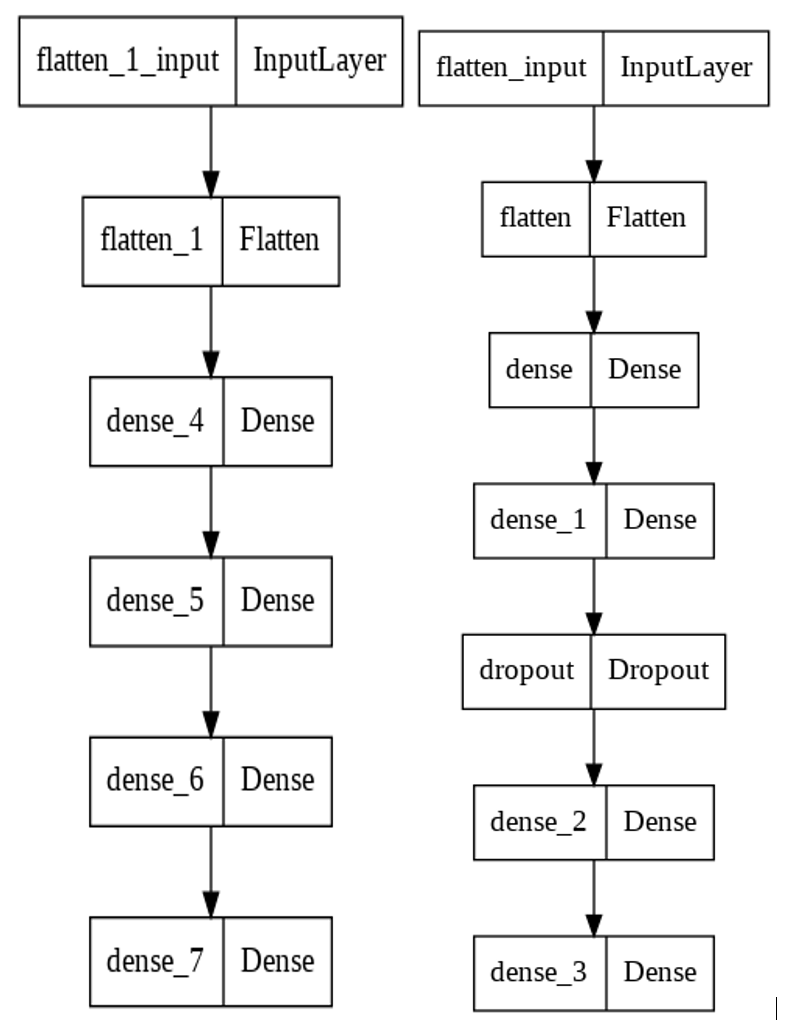
\includegraphics[width=0.5\textwidth]{Capture.PNG}
    \caption{Fashion MNIST Architecture 1 with various trail run}
    \label{fig:compute}
\end{figure}

In the second model architecture following changes were made in the existing model. A few more hidden layers were added and a variation in drop out was made. Use of ReLu activation function, Adam optimizer and variable learning rate was left as it was in architecture 1. Addition of more layers increases the validation accuracy of the model and the drop out layer reduces the over fitting problem like mentioned in the previous architecture. Also, different batch sizes were used for training in this architecture.

\begin{itemize}
    \item \textbf{Trial Run 1:} Four hidden layers in the model were applied with 20\% dropout, 0.0001 learning rate and beta of 0.95 and L2 regularization was applied at every dense layer. 
    \item \textbf{Trial Run 2:} In this trial, dropout was changed to 50\%, learning rate was increased to 0.0005 and L regularization was applied to every dense layer.
    \item \textbf{Trial Run 3 and 4:} In the last two trials we wanted to see what difference batch size makes in performance, so model was trained with two different batch size i.e., 32 and 64 with a learning rate of 20\%.
\end{itemize}

\begin{figure}[H]
    \centering
    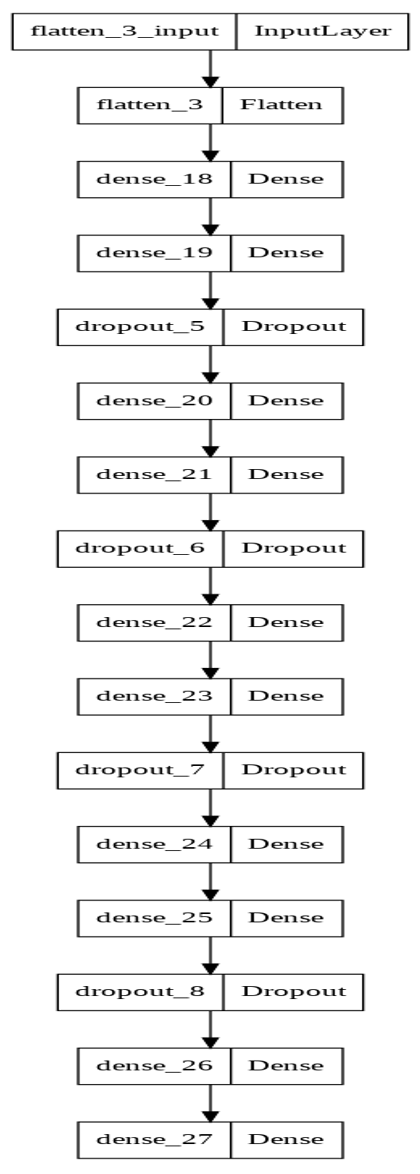
\includegraphics[with=\textwidth, height = 19cm]{Capture1.png}
    \caption{Fashion MNIST architecture 2 with various trail run}
    \label{fig:MNISTAc2}
\end{figure}

\subsection{CIFAR-100 dataset}

For classification of CIFAR-100, we tried three different architectures based on convolution neural networks, to observe changes in model's performance and efficiency.

\begin{itemize}
    \item \textbf{First:} We implement the simplest architecture with two convolution , max-pooling layers continued with a Flatten and two dense layers respectively.
    \item \textbf{Second:} Convolutional architecture were implemented with a residual block.
    \item \textbf{Third:} Deeper Convolutional architecture were implemented with a residual block and a bottleneck in series. 
\end{itemize}

The fig. \ref{fig:Cifar100A1} shows our first architecture. This is the simplest sequential architecture model with two convolution layers, two max-pooling layers and two fully connected layers at the end. In the first convolution we are using 32 filters with kernel size of (3, 3) followed by max-pooling layers. In the following convolutional layer 64 filters of same kernel size were used with pooling layers. Finally, two dense layers with 100 nodes each were added. In this architecture we wanted to see how well the model performs with the simplest possible architecture.

\begin{figure}[H]
    \centering
    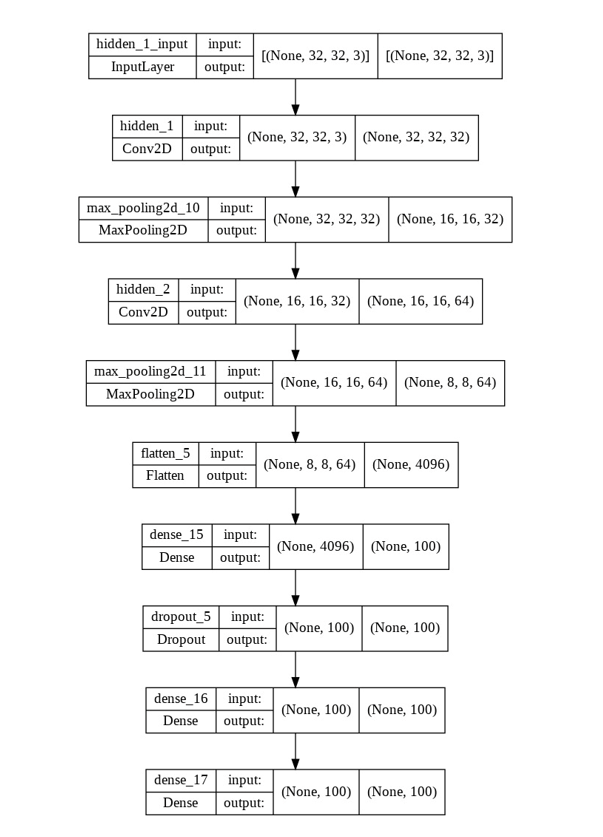
\includegraphics[with=\textwidth]{Capture2.png}
    \caption{CNN Architecture 1 for CIFAR-100}
    \label{fig:Cifar100A1}
\end{figure}

In the second architecture shown in fig. \ref{fig:Cifar100A2} we decided to add more convolution layers in sequential mode. In total, we added 7 more convolution layers and 6 more max-pooling layers to our predefined architecture. With this architecture we were trying to observe whether we can improve the performance by adding more sequential layers. We also added linear regularization l2 and dropout layers for further regularization.

\begin{figure}[H]
    \centering
    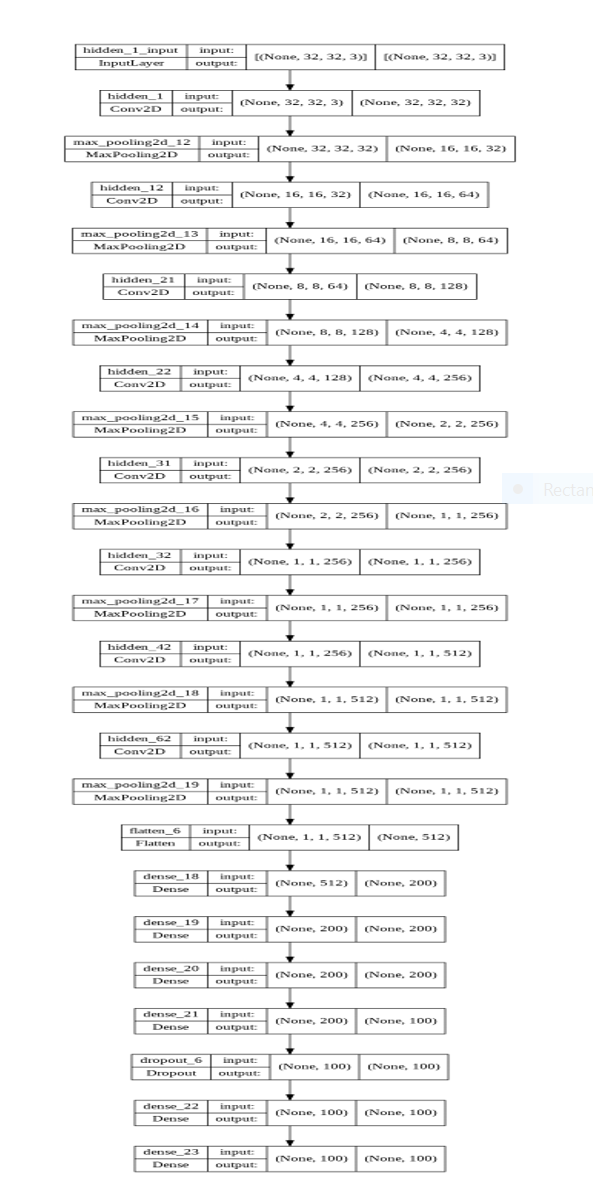
\includegraphics[with=\textwidth, height = 20cm]{Capture3.PNG}
    \caption{CNN Architecture 2 for CIFAR-100}
    \label{fig:Cifar100A2}
\end{figure}

In the final architecture we tried to implement simplest residual architecture as shown in fig. \ref{fig:Cifar100A3}. In this architecture we tried to implement one residual architecture and one bottleneck architecture in series to check how well the model performs in comparison to the previous two models. Figures \ref{fig:ResidualB} and fig. \ref{fig:ResidualBConv} show the flowcharts of residual block, here the skip connection jumps over some layers. Skipping the layers in the initial training stages effectively simplifies the network. This speeds the learning pace by reducing the vanishing gradient problem. In our model we are skipping two convolution layers and two batch normalization layers by each feed-forward. We implemented this architecture to see if our lower validation accuracy is due to the vanishing gradient problem.

\begin{figure}[H]
    \centering
    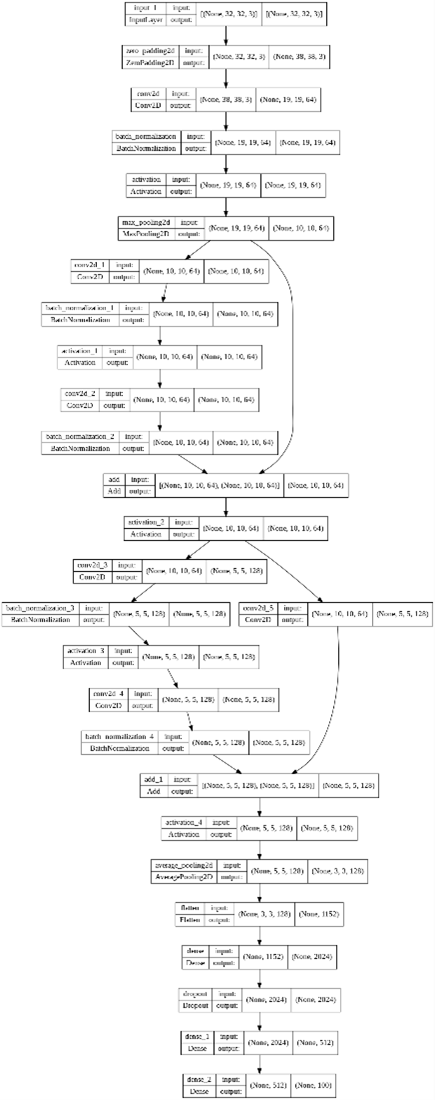
\includegraphics[with=\textwidth, height=20cm]{Picture1.png}
    \caption{CNN Architecture 3 for CIFAR-100}
    \label{fig:Cifar100A3}
\end{figure}

\begin{figure}[H]
    \centering
    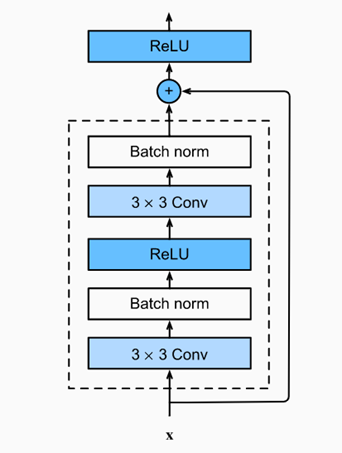
\includegraphics[with=\textwidth, height=8cm]{Picture2.png}
    \caption{Residual Architecture}
    \label{fig:ResidualB}
\end{figure}

\begin{figure}[H]
    \centering
    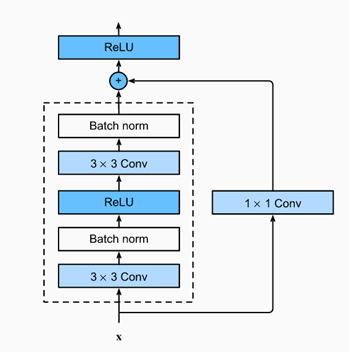
\includegraphics[with=\textwidth, height=8.5cm]{Picture3.png}
    \caption{Residual Architecture with Convolution}
    \label{fig:ResidualBConv}
\end{figure}


The model architecture that achieved the best validation accuracy for CIFAR-100 dataset was the model based on residual architecture. Notable changes in training efficency were observed in comparison between the three architectures but no significant changes in the validation efficiency were observed.

\section{Experimental Setup}
\subsection{Fashion MNIST dataset}

For the experimental setup of the Fashion MNIST datasets, initially the data was imported from TensorFlow datasets API. As Fashion MNIST dataset contains about 70,000 images in total, these datasets were divided into 85\% of training sets and 15\% of testing sets. During the preprocessing process the pixel value of training images and testing images were divided by 255 to convert them to one-hot vector. Then, it is followed by model architecture one and module architecture two with change of different hyperparameters as described in approaches.

\begin{table}[h]
 \caption{Summary of hyperparameters used for Fashion-MNIST}
    \begin{tabular}{|c|c|c|c|c|c|} \hline
      Model   & Hidden Layers & Dropout & L2 Regularization & Learning Rate & Batch size\\
    Arch1 TR1 & 3 & 0 & Not used & 0 & 32\\
    Arch1 TR2 & 3 & 0.2 & Used & 0.001 & 32\\
    Arch1 TR3 & 3 & 0.05 & Used & 0.001 & 32\\ 
    Arch1 TR4 & 3 & 0.05 & Used & 0.0001 & 32\\
    Arch2 TR1 & 9 & 0.2 & Used & 0.0001 & 32\\
    Arch2 TR2 & 9 & 0.5 & Used & 0.0005 & 32\\
    Arch2 TR3 & 9 & 0.2 & Used & 0.0005 & 32\\
    Arch2 TR4 & 9 & 0.2 & Used & 0.0005 & 64\\\hline
    \end{tabular}
 
    \label{tab:CNN-perf}
\end{table}

\noindent Note : 200 neurons were used in each Train Run in the above mentioned architectures.

\subsection{CIFAR-100 dataset}
We used Keras API to load the data and train the model. The dataset was initially divided into 9:1 training and validation sets. The labels were converted into one hot encoded vectors. The first architecture was run several times using different learning rates and regularization for 50 epochs, other two architectures were run for once, and results were noted. We used Adam optimizer for optimization and categorical cross entropy as the loss function. All the layers in architecture 2 and three were regularized with L2 regularization and a 40\% dropout layer was also implemented in between two dense layers.

\section{Experimental Results}
\subsection{FMNIST Dataset}
Complete details of hyperparameters used for Fashion-MNIST dataset is stored in Table \ref{tab:CNN-perf} \newline
The experimental result for the FMNIST dataset with various trial run is given as follows:
\vspace{5 mm}
\newline
\textbf{Model Architecture 1}
\subsubsection{Trial Run 1}

Figures \ref{fig:Arch1_Tr1} compares training & testing accuracy and also training & testing loss for Trial Run1. Training accuracy 94.33\% and validation accuracy 88.79\% with no dropout layers and no L2 regularization. In a comparable way, training loss 0.1515 and validation loss 0.50. From trial run 1, inference can be drawn that validation decreases while training increases due to overfitting problem. Therefore, some sort of regularization is needed to alleviate this problem.

\begin{figure}[H]
    \centering
    \subfloat{{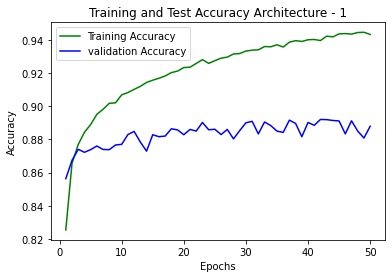
\includegraphics[width=0.465\textwidth]{Arch1_TR1(a).png} }}%
    \qquad
    \subfloat{{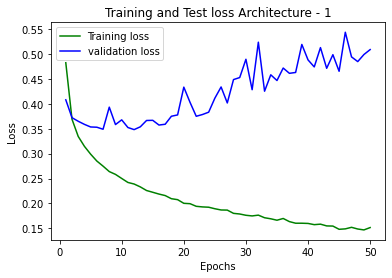
\includegraphics[width=0.465\textwidth]{Arch1_TR1(b).png} }}%
    \caption{Training vs validation accuracy and Loss curve for Arch 1 TR1}%
    \label{fig:Arch1_Tr1}%
\end{figure}

\subsubsection{Trial Run 2}
Figures \ref{fig:Arch1_Tr2} describe the variation in training loss vs testing accuracy and training vs testing loss values respectively when dropout of 0.2 and L2 regularization were added with a learning rate of 0.001. Figure \ref{fig:Arch1_Tr2}
\begin{table}[h]
\centering
\caption{Results for Architecture 1 Trial Run 2}
\begin{tabular}{|l|l|}
\hline
Training Accuracy   & 71.06\% \\ \hline
Validation Accuracy & 71.78\% \\ \hline
Training Loss        & 1.3532    \\ \hline
Validation Loss     & 1.3277    \\ \hline
\end{tabular}
\end{table}

\begin{figure}[H]
    \centering
    \subfloat{{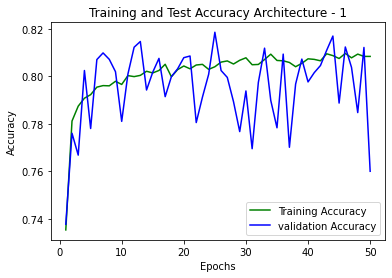
\includegraphics[width=0.465\textwidth]{Arch1_TR2(a).png} }}%
    \qquad
    \subfloat{{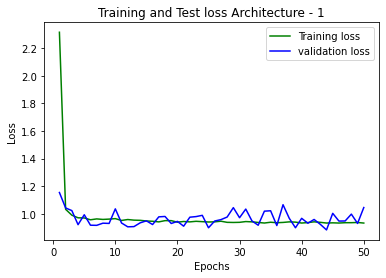
\includegraphics[width=0.465\textwidth]{Arch1_TR2(b).png} }}%
    \caption{Training vs validation accuracy and Loss curve for Arch 1 TR2}%
    \label{fig:Arch1_Tr2}%
\end{figure}

\subsubsection{Trial Run 3}
In trail run 3, dropout was reduced to 0.05 and only L2 regularization was applied with a learning rate of 0.001. From the result, we can see validation accuracy and training accuracy of the model is improved and there is considerable reduction in training loss and validation loss. The results plotted in fig. \ref{fig:Arch1_Tr3} state that an increase in accuracy were observed with a change in hyperparamters as mentioned in the Trial Run 3.

\begin{table}[h]
\centering
\caption{Results for Architecture 1 Trial Run 3}
\begin{tabular}{|l|l|}
\hline
Training Accuracy   & 87.16\% \\ \hline
Validation Accuracy & 85.26\% \\ \hline
Training Loss        & 0.41    \\ \hline
Validation Loss     & 0.48    \\ \hline
\end{tabular}
\end{table}

\begin{figure}[H]
    \centering
    \subfloat{{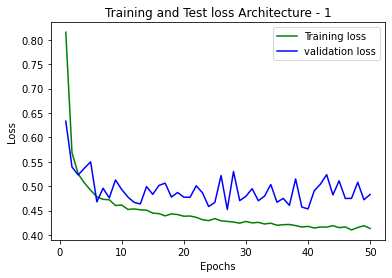
\includegraphics[width=0.465\textwidth]{Arch1_TR3(a).png} }}%
    \qquad
    \subfloat{{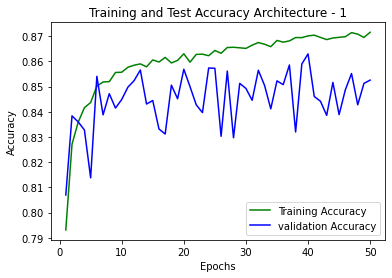
\includegraphics[width=0.465\textwidth]{Arch1_TR3(b).png} }}%
    \caption{Training vs validation accuracy and Loss curve for Arch 1 TR3}%
    \label{fig:Arch1_Tr3}%
\end{figure}


\subsubsection{Trial Run 4}
In fourth trail run we changed the learning rate to 0.0001 which made the optimization much smoother but in 50 epochs, we can only get up to 80.23\% training accuracy and even lower validation accuracy.

\vspace{5 mm}
\newline
\noindent \textbf{Model Architecture 2}

\subsubsection{Trial Run 1}
In model architecture 2 Trial 1, a dense layer was applied with dropout of 20\%, learning rate of 0.0001 and L2 regularization in every dense layer with beta (average momentum) to be 0.95. Results for Training and Testing accuracy could be viewed in Figure \ref{fig:Arch2_Tr1}.

\begin{table}[h]
\centering
\caption{Results for Architecture 2 Trial Run 1}
\begin{tabular}{|l|l|}
\hline
Training Accuracy   & 94.86\% \\ \hline
Validation Accuracy & 89.06\% \\ \hline
Training Loss        & 0.19    \\ \hline
Validation Loss     & 0.4    \\ \hline
\end{tabular}
\end{table}


\begin{figure}[H]
    \centering
    \subfloat{{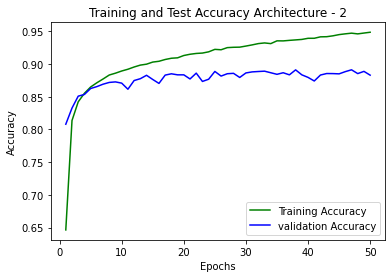
\includegraphics[width=0.47\textwidth]{Arch2_TR1(a).png}}}%
    \qquad
    \subfloat{{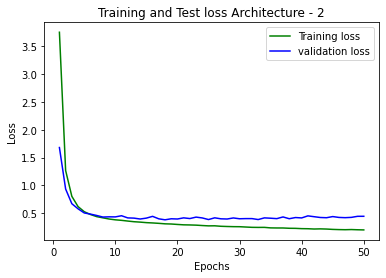
\includegraphics[width=0.47\textwidth]{Arch2_TR1(b).png}}}%
    \caption{Training vs validation accuracy and Loss curve for Arch 2 TR1}%
    \label{fig:Arch2_Tr1}%
\end{figure}

\subsubsection{Trial Run 2}
In the second model architecture, trial 2, a learning rate of 0.0005 was applied with 50\% dropout and L2 regularization on every layer, fig.\ref{fig:Arch2_Tr2} shows the performances with these changes.

\begin{table}[h]
\centering
\caption{Results for Trial Run 2}
\begin{tabular}{|l|l|}
\hline
Training Accuracy   & 91.10\% \\ \hline
Validation Accuracy & 89\% \\ \hline
Training Loss        & 0.3    \\ \hline
Validation Loss     & 0.4    \\ \hline
\end{tabular}
\end{table}

\begin{figure}[H]
    \centering
    \subfloat{{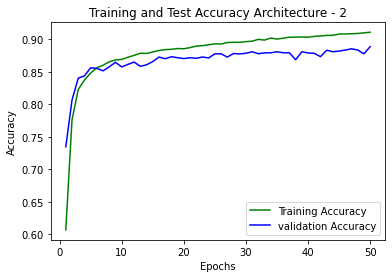
\includegraphics[width=0.47\textwidth]{Arch2_TR2(a).png}}}%
    \qquad
    \subfloat{{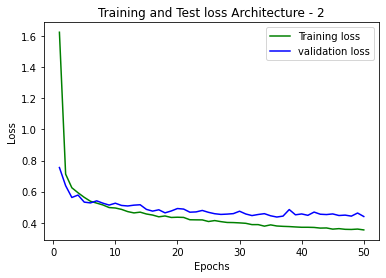
\includegraphics[width=0.47\textwidth]{Arch2_TR2(b).png}}}%
    \caption{Training vs validation accuracy and Loss curve for Arch 2 TR2}%
    \label{fig:Arch2_Tr2}%
\end{figure}

\subsubsection{Trial Run 3 and 4}
In trial run 3 and trial run 4, for model architecture 2, everything remained same as in Trial Run 2 but this time we introduced batch size of 32 and 64, and Dropout of 20\%. respectively.

\begin{table}[h]
\centering
\caption{Results for Trial Run 3 and 4}
\begin{tabular}{|l|l|}
\hline
Training Accuracy   & 90.22\% \\ \hline
Validation Accuracy & 87.82\% \\ \hline
Training Loss        & 0.37    \\ \hline
Validation Loss     & 0.45    \\ \hline
\end{tabular}
\end{table}

\begin{figure}[H]
  \centering
    \subfloat{{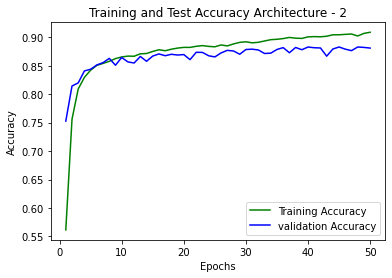
\includegraphics[width=0.47\textwidth]{Arch2_TR3(a).png}}}%
    \qquad
    \subfloat{{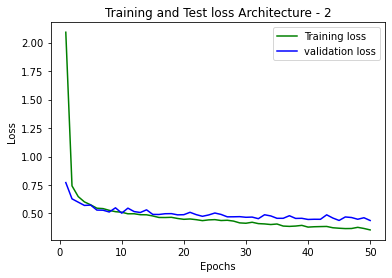
\includegraphics[width=0.47\textwidth]{Arch2_TR3(b).png}}}%
    \caption{Training vs validation accuracy and Loss curve for Arch 3 TR2}%
    \label{fig:Arch2_Tr3}%
\end{figure}
On comparison of Trial Run 3 and 4 where different batch size were used. We do not see a significant difference in both accuracy and loss scores observed in the two cases.

\subsubsection{Confusion Matrix for the Best model}
A confusion matrix is a summary of prediction results on a classification problem. The number of correct and incorrect predictions are summarized with count values and broken down by each class. We plotted the confusion matrix for Fashion-MNIST dataset using scikit-learn library.

\begin{figure}[H]
    \centering
    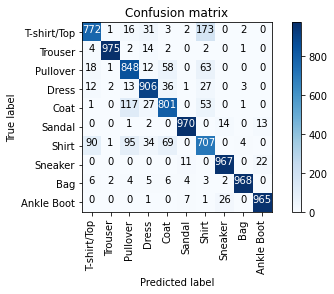
\includegraphics[with=\textwidth]{ConfMatrix.png}
    \caption{Confusion Matrix for best model}
    \label{fig:ConfMatrix}
\end{figure}

\subsection{CIFAR-100 Dataset}
\subsubsection{First Architecture}
In the first architecture, we tried two different learning rates 0.01 and 0.0001. The highest validation accuracy of 0.3 and the lowest validation loss of 2.5 was noted for 0.01 learning rate. fig. \ref{fig:Arch1_CNN(a)} and fig. \ref{fig:Arch1_CNN(b)}

\begin{table}[h]
\centering
\caption{Results for Trial Run 3 and 4}
\begin{tabular}{|l|l|l|}
\hline
Learning rate & 0.01 & 0.0001 \\ \hline
Training Accuracy   & 50\% & 25\% \\ \hline
Validation Accuracy & 30\% & 22\%\\ \hline
Training Loss        & 1.6 & 3.19 \\ \hline
Validation Loss     & 2.5 & 3.11 \\ \hline
\end{tabular}
\end{table}

\begin{figure}[H]
    \centering
    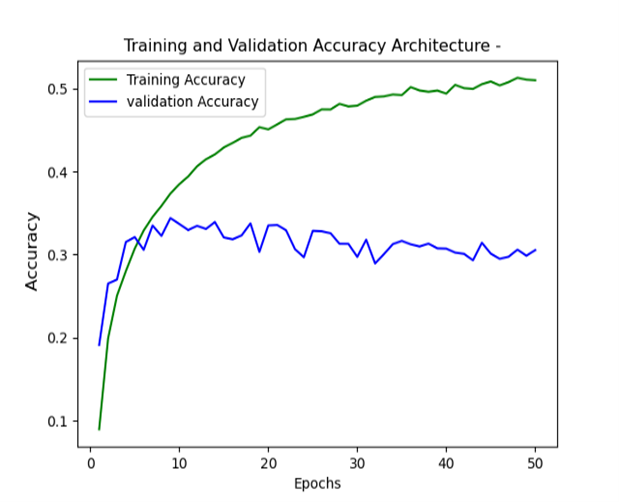
\includegraphics[with=\textwidth]{Conv1_Arch1(b).png}
    \caption{Architecture 1 for CIFAR-100 with LR 0.01}
    \label{fig:Arch1_CNN(b)}
\end{figure}

\begin{figure}[H]
    \centering
    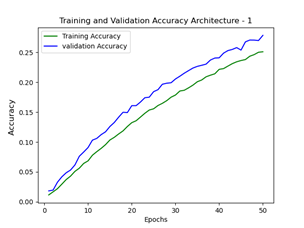
\includegraphics[with=\textwidth]{Conv1_Arch1(a).png}
    \caption{Architecture 1 for CIFAR-100 with LR 0.0001}
    \label{fig:Arch1_CNN(a)}
\end{figure}

\subsubsection{Second Architecture}
In the second module architecture, seven more convolution layers were added including six max pooling layer, L2 linear regularization and dropout of 40\% were added into the model. We obtained the following results: fig. \ref{fig:Arch2_CNN}

\begin{table}[h]
\centering
\caption{Results for Trial Run 3 and 4}
\begin{tabular}{|l|l|}
\hline
Training Accuracy   & 61\% \\ \hline
Validation Accuracy & 39\% \\ \hline
Training Loss        & 1.5    \\ \hline
Validation Loss     & 2.6    \\ \hline
\end{tabular}
\end{table}

\begin{figure}[H]
    \centering
    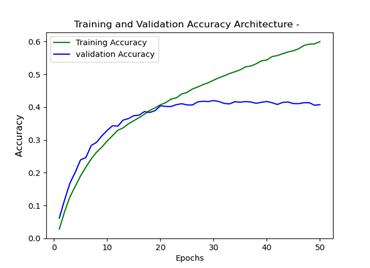
\includegraphics[with=\textwidth]{Conv_arch2.png}
    \caption{Architecture 2 for CIFAR-100}
    \label{fig:Arch2_CNN}
\end{figure}

The above figure shows, training accuracy increases and reach up to 61\% while validation accuracy increases up to 40\% and becomes flatten. This shows even having a smaller learning rate and adding regularization could not solve the problem of overfitting. 


\subsubsection{Third Architecture}
In third architecture, one residual block and one bottleneck layer were added, the training accuracy rose to 90\% in just 15 epochs, but validation accuracy was still lower as shown in the fig. \ref{fig:Arch3_CNN}

\begin{table}[h]
\centering
\caption{Results for Trial Run 3 and 4}
\begin{tabular}{|l|l|}
\hline
Training Accuracy   & 95\% \\ \hline
Validation Accuracy & 42\% \\ \hline
Training Loss        & 0.95 \\ \hline
Validation Loss     & 3.11  \\ \hline
\end{tabular}
\end{table}

\begin{figure}[H]
    \centering
    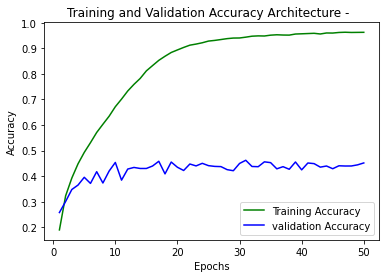
\includegraphics[with=\textwidth]{Conv_Arch3.png}
    \caption{Architecture 3 for CIFAR-100}
    \label{fig:Arch3_CNN}
\end{figure}

 We come to conclusion that the model could perform better with increasing the number of images in the datasets.

\subsubsection{Confusion Matrix for the Best model}
A confusion matrix is a summary of prediction results on a classification problem. The number of correct and incorrect predictions are summarized with count values and broken down by each class. We plotted the confusion matrix for CIFAR-100 dataset using scikit-learn library.

\begin{figure}[H]
    \centering
    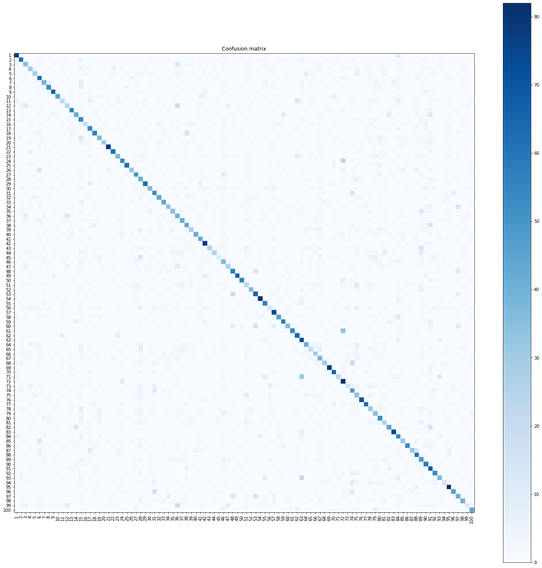
\includegraphics[with=\textwidth]{Conf_Matrix_Cifar100.png}
    \caption{Confusion Matrix for CIFAR-100 best model}
    \label{fig:Conf_matrix_Cifar100}
\end{figure}

\section{Discussion}
\subsection{FMNIST Dataset}

For FMNIST dataset, we began with a simple architecture including only four dense layers. We trained the model for 50 epochs without use of any regularization and hyper-parameters at first and the results obtained were 88.79\% & 94.33\% for validation and training accuracy. Similarly, the losses were 0.1515 & 0.5 for training and validation. From this result, we saw that the model is over-fitting and so, we applied regularization techniques in our architecture. We made use of L2 regularization and added a dropout layer in which 20\% of total neurons used in training were laid off during training phase. The changes made in the later adversely affect the trainng of the model and suffer over regularization. Similarly, in the third trail run we changed the dropout percentage to 50\% and used L2 regularization only. This improved our training and validation accuracy to 87.6\% & 85\% respectively. In our fourth trail run we changed the learning rate to 0.0001 which made the optimization much smoother but in 50 epochs, we can only get up to 80.23\% training accuracy and even lower validation accuracy.
With all these observations, we used more hidden layers in the model to get higher accuracy. From the second architecture we choose to use a dropout of 20\%,  with the learning rate 0.0001 and beta (average momentum) of 0.95. We also added L2 regularization on every dense layer and with these hyper-parameters, we get training accuracy of 94.86\% and validation accuracy 89\% and similar type of trend in validation and training loss. In the results section, the loss vs epoch shows that the learning as well as validation curves are exceptionally smooth and not escalating that much. Similarly, we changed the batch size to 32 and 64 in Trial Run 3 & 4. The training and validation accuracy were almost similar in both runs. Therefore, changing the batch size does not make that much of a difference.  

\subsection{CIFAR-100 Dataset}
For this dataset, we used two different learning rates with the first architecture. To begin with, we used a learning rate of 0.01 which gave a training accuracy of 50\% but the validation accuracy could not get past 30\%. Validation accuracy increased for the first 10 epochs then began to decline. We concluded that 0.01 might be a high learning rate for this architecture. We lowered the learning rate down to 0.0001 and observe that both the training and validation accuracies were showing a smooth incline but only up to 25\% and 22\% respectively. After this, we proposed a new deeper architecture deeper. We used L2 regularization along with 40\% dropout between dense layers. It produced an accuracy of 61\% on the training set and 39\% on the validation data. It seemed to be performing well initially but after some epochs the accuracy graph flattened out. We hypothesized that adding residual blocks to the architecture might accelerate the learning process. In the third architecture where we used a residual network with a bottle neck layer, results show that it helps the model to perform exceptionally well on Training dataset. On testing the trained model using this architecture on Validation dataset, shows that model is overfitting on already learned data during training and does not generalises well on unseen data. From the results in fig. \ref{fig:Arch3_CNN}, it turned out to be helpful as the training accuracy rose to 90\% in just 15 epochs, but validation accuracy was still low. In all these trial runs, we got to a point where even having a smaller learning rate and adding regularization could not solve the problem of overfitting. We concluded that the training dataset is not big enough for these architectures to get to a higher accuracy.


\section{Conclusions}

The programming endeavour achieved in this homework, helped us understand the applicability and practical application of the hyper-parameters learnt in class lectures and Hackathons during this course. The sequential steps in the homework assisted us in realizing the intuition behind the tuning/tweaking of hyperparameters and how they can be fitted in a neural network to create a model with higher generalizing power. The results obtained above justify that application of dropout helps us reduce the overfitting problem. We developed neural networks for Fashion MNIST and Cifar 100 dataset in our work. After working on these datasets we come to conclusion that neural networks consiting of only fully connected layers could perform well and can be used to develop models with higher training and validation accuracies ~90\%. This is possible due to the less categorically diverse large dataset in case of the prior as compared to later in neural network model development. On training Cifar 100 dataset using convolutional layers that helps to perform training using feature extraction process from the input images. The trained model in this case, finds it hard to genralize well on unseen data during testing is due to the highly diverse and presence of fewer images per category in the Cifar 100 dataset. Even use of residual blocks in the convolutional layers make it hard to resolve the overfitting problem. Further work needs to be conducted  using transfer learning with pre-trained models like InceptionV3 or VGG-19 that are already trained on larger data sets can be used to attain higher accuracy and better results could be obtained on already trained neural networks.


\begin{table}[h]
    \caption{Contributions by team member for this assignment.}
    \centering
    \begin{tabular}{|c|c|} \hline
    {\bf Team Member}     &  {\bf Contribution}  \\ \hline
    Shubham Bery     &   Coding and results visualization \\
    Shiva Paudel     &   Coding and results interpretation \\
    Puranjit Singh   &   Idea formulation and report writing \\ 
    Kantilata Thapa  &   Idea formulation and report writing \\ \hline
    \end{tabular}
    \label{tab:contribution}
\end{table}

\bibliographystyle{plainurl}
\bibliography{main}
[1] Saha S., "A Comprehensive Guide to Convolutional Neural Networks", 2018
[2] Mahajan, P., "Fully Connected vs Convolutional Neural Networks", 2020
[3] He, K.; Zhang, X.; Ren, S.; Sun, J.; "Spatial pyramid pooling in deep convolutional networks for visual recognition. IEEE transactions on pattern analysis and machine intelligence", 37(9), 1904-1916, 2015\newline
[4] Xiao, H.; Rasul, K.; Vollgraf, R.; "Fashion-MNIST: a Novel Image Dataset for Benchmarking Machine Learning Algorithms. 1–6. Retrieved from.", 2017\newline
[5] Lei F. F.; "https://cs231n.github.io/convolutional-networks/#overview", 2021
 
\end{document}